\documentclass[letterpaper,10pt]{article}

%\setlength{\parindent}{0in}
%\usepackage{fullpage} 
\usepackage{amsmath}
\usepackage{amssymb}
\usepackage{enumerate}
\usepackage{graphicx}
\usepackage{color}
\usepackage[table]{xcolor}
\usepackage{dcolumn}
\oddsidemargin 0.0in
\textwidth 6.5in 
\newcolumntype{.}{D{.}{.}{-1}}
\newcommand*{\myalign}[2]{\multicolumn{1}{#1}{#2}}

% Project Assignment 4 OMOE and Risk is due 3/2/12. It is a team event. Please 
% see the Project area in Sakai for more guidance.
% Overall Measure of Effectiveness (OMOE):
% a) Calculate the overall measure of effectiveness (OMOE) of the alternative IED 
% robots.
% b) Given variant D information, investigate the LOE test data, and analyze the 
% data for the mean, range, and variance and other aspects, as desired, with 
% respect to KPP threshold and goal values.
% c) Use box plots or other methods and tools, as needed, to provide a graphical 
% view of the test data, and evaluate the data variation in the context of the 
% alternative selection process.
% d) Select a best robot prototype variant based solely on OMOE and your 
% assessment of the test data.
% e) Summarize and present the results of your analysis.
% Risk Analysis:
% a) Use one of the risk analysis methods described in class to create a risk 
% assessment for each of the prototype variants.
% b) Conduct a risk assessment for the overall product, in general.
% c) Identify ways to mitigate the risk.
% d) Summarize and present the results of your analysis.
% Remember to complete your RPG Role Evaluation on the Discussion Board 
% also!

\title{Project 4 \\ \Large Team CLEAR \\ \normalsize (\textcolor{red}{C}onvoy \textcolor{red}{L}evel \textcolor{red}{E}xplosive \textcolor{red}{A}mmunition \textcolor{red}{R}emoval)}
\author{Christian Aall: Testing \& Evaluation \\ 
	Steve Mazza: Team Lead \\ 
	Michael Oexmann: Analyst \\ 
	Elizabeth Swisher: Lead Systems Engineer} 
	
\date{March 2, 2012}

\begin{document}
\maketitle
\tableofcontents
\listoftables
\listoffigures

\pagebreak

\section{Overall Measures of Effectiveness Analysis}
\subsection{Analysis of Alternative IED Robots}
The next step in moving towards an educated and well-supported recommendation for continued prototype development is to compare the Overall Measures of Effectiveness (OMOEs) for each robot variant. These values were determined through the comparison of raw test data converted into \emph{scaled scores} with weight input from the Quality Function Deployment (QFD) diagrams. The OMOE calculated results for each of the each of the alternative robots is shown in Table \ref{tab:IEDanalysis}.

\begin{table}[h!tbp]\scriptsize
	\begin{center}
		\begin{tabular}{c..........}
			\hline
			& \myalign{p{1.1cm}}{\begin{center}\tiny\textbf{Mission Reliability}\end{center}} 
			& \myalign{p{1.1cm}}{\begin{center}\tiny\textbf{Operational Availability}\end{center}}
			& \myalign{p{1.1cm}}{\begin{center}\tiny\textbf{Vehicle Weight}\end{center}}
			& \myalign{p{1.1cm}}{\begin{center}\tiny\textbf{Vehicle Drop Height}\end{center}}
			& \myalign{p{1.1cm}}{\begin{center}\tiny\textbf{Refueling Time}\end{center}}
			& \myalign{p{1.1cm}}{\begin{center}\tiny\textbf{DRM Elapsed Time}\end{center}}
			& \myalign{p{1.1cm}}{\begin{center}\tiny\textbf{Deployed-to-Ready Time}\end{center}}
			& \myalign{p{1.1cm}}{\begin{center}\tiny\textbf{SMETAL-V Storage Container}\end{center}}
			& \myalign{p{1.1cm}}{\begin{center}\tiny\textbf{Operational Team Size}\end{center}} 
			& \myalign{p{1.1cm}}{\begin{center}\tiny\textbf{OMOE}\end{center}} \\
			\hline\hline
			\rowcolor{yellow} & 0.248 & 0.289 &	0.000 &	0.097 &	0.067 &	0.064 &	0.137 &	0.060 &	0.037 &	1.000 \\
			A & 0.40 & 1.00 &	0.50 &	1.00 &	0.39 &	0.39 &	0.59 &	0.29 &	1.00 &	0.672 \\
			B & 0.80 & 0.80 &	1.00 &	0.00 &	0.28 &	0.66 &	0.39 &	0.17 &	0.00 &	0.554 \\
			C & 0.80 & 1.00 &	0.00 &	1.00 &	0.70 &	0.18 &	0.70 &	0.13 &	1.00 &	0.783 \\
			D & 1.00 & 1.00 &	0.25 &	1.00 &	0.83 &	0.87 &	0.79 &	0.17 &	1.00 &	0.902 \\
			\hline
		\end{tabular}
	\end{center}
	\caption{Calculated OMOEs for each robot variant}
	\label{tab:IEDanalysis}
\end{table}

Based on the results, variant $D$ has achieved the highest OMOE.
\subsection{Analysis of Variant D}
Consistent with previously conducted analysis of prototype variants, the Limited Objective Exercise (LOE) test results for variant $D$ have been compared to Key Performance Parameters (KPPs) using Analysis of Variance (ANOVA) methods. Similar to previous variant analyses, the ANOVA focused on comparison to KPP goal values vs. threshold values due to the variant's ability to meet or exceed thresholds.  The results of this analysis can be seen in Table \ref{tab:Danalysis}.

\begin{table}[h!tbp]
	\begin{center}
		\begin{tabular}{lrr....}
			\myalign{c}{\large\textbf{Summary}} & & & & & & \\
			\hline
			\myalign{c}{\textbf{Groups}} 
			& \myalign{c}{\textbf{Count}} 
			& \myalign{c}{\textbf{Average}} 
			& \myalign{c}{\textbf{Variance}} & & \\
			\hline\hline
			Goal &	9 &	\myalign{.}{177.85} &	19.76 &	1503.40 & & \\
			Var D &	9 &	\myalign{.}{267.4192814} &	29.71 &	4205.52 & &	\\
			\hline
			\vspace*{3mm} & & & & & & \\
			\myalign{c}{\large\textbf{ANOVA}} & & & & & & \\
			\myalign{c}{\textbf{Source of Variation}} 
			& \myalign{c}{\textbf{SS}} 
			& \myalign{c}{\textbf{df}} 
			& \myalign{c}{\textbf{MS}} 
			& \myalign{c}{\textbf{F}} 
			& \myalign{c}{\textbf{p-value}} 
			& \myalign{c}{\textbf{F crit}} \\
			\hline\hline
			Between Groups &	445.70 &	1 &	445.70 &	0.16 &	\cellcolor{yellow}0.70 &	4.49 \\
			Within Groups &	45671.37 &	16 &	2854.46 & & &	\\
			\hline
			Total &	46117.08 &	17 & & & & \\				
			\hline
		\end{tabular}
	\end{center}
	\caption{ANOVA results �- variant D vs. KPP goals}
	\label{tab:Danalysis}
\end{table}
\subsection{Graphical Analysis}
As indicated in the box plots (see Figures \ref{fig:missionReliability} - \ref{fig:deployedToReadyTime} in Appendix \ref{sec:boxPlot} beginning on page \pageref{fig:missionReliability}), variant $D$ exhibits significantly more consistent results than other variants' test data analyzed previously. The fact that the inter-quartile range is relatively small, and that the high and low box plot tails (indicating maximum and minimum values) are short, illustrates more confidence in further test data to exhibit similar results. Most importantly, one will notice that variant $D$ also performed better than previous variants, exhibiting results that much more closely meet the goal values for the KPPs. In summary, the customer may be certain that variant $D$ will perform close to the goal values more consistently, ensuring that mean performance will be higher than variants $A$, $B$, and $C$.

To further strengthen our preliminary decision that variant $D$ is the most desirable and highest performing prototype variant, OMOE data was investigated (see Figures \ref{fig:operationalAvailability} -- \ref{fig:operationalTeamSize} in Appendix \ref{sec:omoe} beginning on page \pageref{fig:operationalAvailability}). The OMOE data reflected that variant $D$ scored the highest in all Overall Measures of Effectiveness except for vehicle weight. Given that it still surpassed the threshold requirements for the Vehicle Weight KPP, and performed exceedingly well in the other measures of effectiveness, we recommend Variant $D$ for further development.

\subsection{Summary Results}
Variant $D$ is the best option going forward when considering cost as an independent variable. Variant $D$ exhibits the most consistent results out of the four variants analyzed. It was the highest performing alternative when measured against the KPPs. Variant $D$ also was rated very highly in all OMOEs. When considered together, alternative $D$ exhibits the strongest technical performance of the four variants.

\section{Risk Analysis}
\subsection{Risk Assessment by Prototype}
A risk analysis was performed for each of the four prototype variants ($A$, $B$, $C$, and $D$). To measure risk, four system components including the IED sensor, robot power source, robot drive mechanism and openness of architecture, were evaluated.  Risk measurements were based on the probability (or likelihood) of failing to meet performance objectives, and the consequence (or impact) of failing to achieve that outcome.  The results of this analysis can be seen in Figures \ref{fig:riskMetricKey} - \ref{fig:riskAnalysisD} in Appendix \ref{sec:riskAnalysisData}.

A thorough risk analysis indicates variant $D$ as having the lowest amount of risk due to all of its components achieving a risk level rating of \emph{low}. This rating means that the variant has little potential to cause disruption of schedule, increase in cost or performance. The variant with the highest level of risk is variant $A$. This variant's system components all received a risk level rating of \emph{medium}, meaning there is some potential for disruption of schedule, increase of cost or degradation of performance. With close government monitoring of contractor progress, most barriers will be overcome. Variant $B$ and $C$ received very similar ratings having most components fall within the \emph{medium} risk level rating and a single component having \emph{low} risk. 

\subsection{Overall Risk Assessment}
Analyzing the overall risk averaged over each prototype at the component level presents a useful view of risk area. The four components that were analyzed were IED sensor, robot power source, robot drive mechanism, and openness of architecture. Across the four prototypes, the IED sensor has the lowest probability of reaching required technical performance within estimated schedule and cost. The consequence of not meeting the requirements for the IED sensor would result in a moderate reduction in technical performance or supportability with limited impact on program objectives, minor schedule slip, and approximately a 5\% budget increase over the allocated amount for the component. Issues arising in regards to the power source would result in the most manageable set of consequences. Issues that arise in creation of the drive mechanism or openness of architecture both have the potential for significant consequences in technical performance, schedule, and cost. Luckily these are also the components that are least likely to have issues arise. By looking at overall risk at the component level risk mitigation strategies can are easier to pin down.
\subsection{Risk Mitigation}
Hedging risk is an important component of successful deployment of a system. Prototyping the alternatives places these on track towards mitigating risks. Our recommended alternative, alternative $D$, has the highest probability of issues arising for the robot power source used. Since the availability of the power source is highly coupled with design of the system it is providing power to, integrating updates to the power source into the alternative early and often is an important risk mitigating strategy. The component with the highest average probability of issues arising across alternatives is with the IED sensor. Risk associated with the IED sensor is highly related to conditions arising that were not anticipated. By designing tests that have a large coverage area and stress the system towards real life events, design flaws are more likely to be encountered early. Continued prototyping and testing to requirements until risk has become successfully mitigated is the best strategy moving forward across 
\subsection{Summary Results}
After considering level of risk across the four alternatives, alternative $D$ was clearly the least risky option. For alternative $D$, the risk associated with robot drive mechanism and openness of architecture is low. Alternative $D$ did have a 50\% probability of encountering issues with the robots power source but the consequences are minimal and the risk can be further reduced by integrating updates to the power source into the alternative early and often. Despite only having a 30\% chance of issues arising due to the robot's power source, alternative $D$ could encounter a moderate reduction in technical performance or supportability with limited impact on program objectives, minor schedule slip, and approximately a 5\% budget increase over the allocated amount for the component if issues come to fruition. The risk associated with the IED sensor can be further reduced by placing added emphasis on testing for problem areas early so potential issues are known at an early stage. Alternative $D$ offers a comfortable level of risk moving forward.
\appendix
\pagebreak
\section{Box Plot Analysis}
\label{sec:boxPlot}
\begin{figure}[h!tbp]
	\begin{center}
		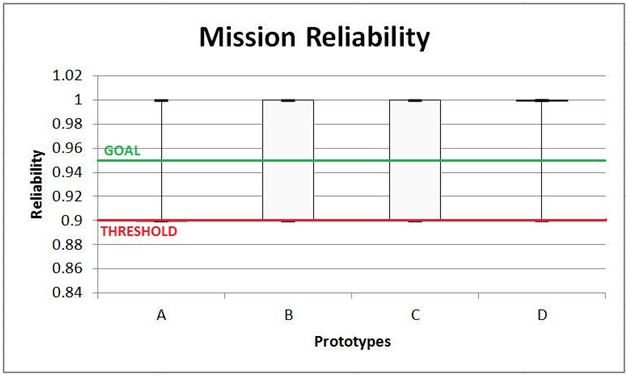
\includegraphics[scale=0.65]{images/missionReliability.png}
	\end{center}
	\caption{Mission reliability data}
	\label{fig:missionReliability}
\end{figure}

\begin{figure}[h!tbp]
	\begin{center}
		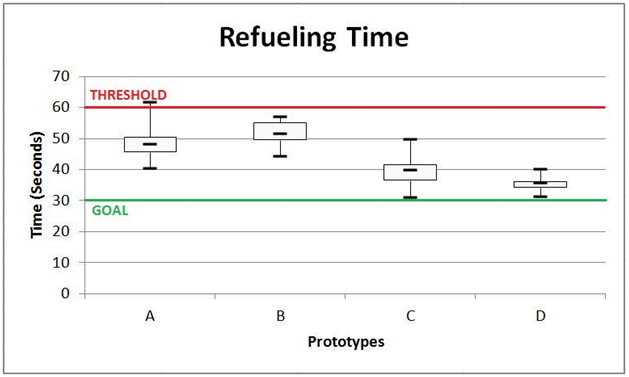
\includegraphics[scale=0.65]{images/refuelingTime.png}
	\end{center}
	\caption{Refueling time data}
	\label{fig:refuelingTime}
\end{figure}

\begin{figure}[h!tbp]
	\begin{center}
		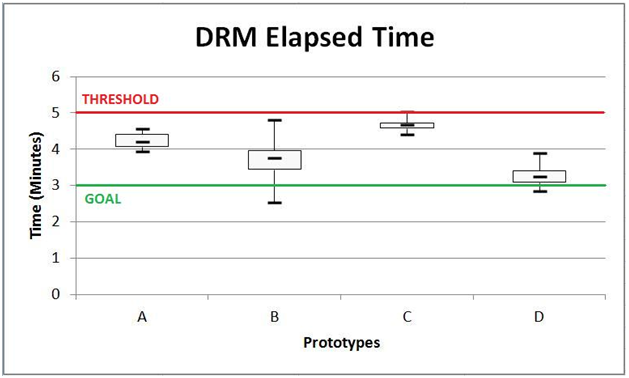
\includegraphics[scale=0.65]{images/drmElapsedTime.png}
	\end{center}
	\caption{DRM elapsed time data}
	\label{fig:drmElapsedTime}
\end{figure}

\begin{figure}[h!tbp]
	\begin{center}
		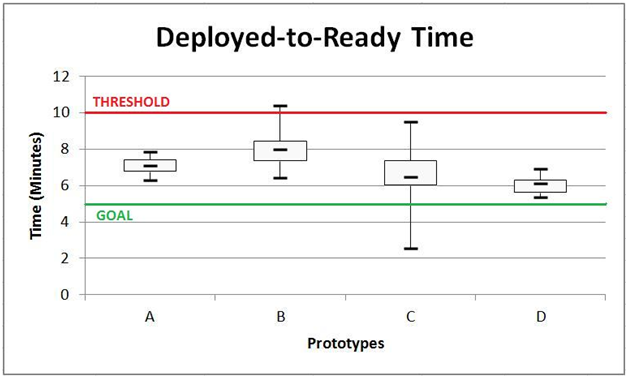
\includegraphics[scale=0.65]{images/deployedToReadyTime.png}
	\end{center}
	\caption{Deployed-to-ready time dat}
	\label{fig:deployedToReadyTime}
\end{figure}
\pagebreak

\section{OMOE Data Analysis}
\label{sec:omoe}
\begin{figure}[h!tbp]
	\begin{center}
		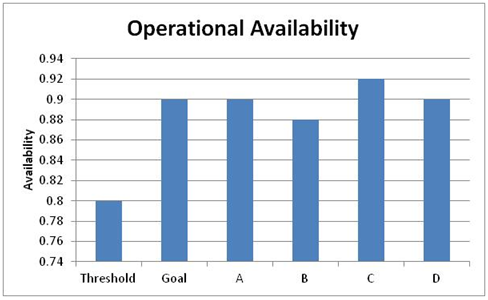
\includegraphics[scale=0.8]{images/operationalAvailability.png}
	\end{center}
	\caption{Operational availability by variant}
	\label{fig:operationalAvailability}
\end{figure}

\begin{figure}[h!tbp]
	\begin{center}
		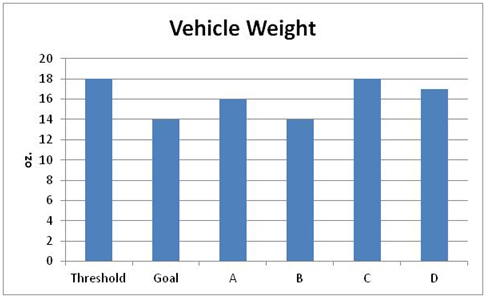
\includegraphics[scale=0.8]{images/vehicleWeight.png}
	\end{center}
	\caption{Vehicle weight by variant}
	\label{fig:vehicleWeight}
\end{figure}

\begin{figure}[h!tbp]
	\begin{center}
		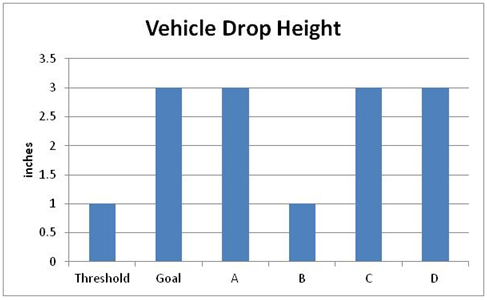
\includegraphics[scale=0.8]{images/vehicleDropHeight.png}
	\end{center}
	\caption{Vehicle drop height by variant}
	\label{fig:vehicleDropHeight}
\end{figure}

\begin{figure}[h!tbp]
	\begin{center}
		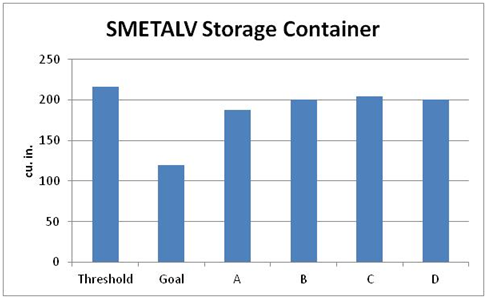
\includegraphics[scale=0.8]{images/smetalvStorageContainer.png}
	\end{center}
	\caption{SMETAL-V storage container volume by variant}
	\label{fig:smetalvStorageContainer}
\end{figure}

\begin{figure}[h!tbp]
	\begin{center}
		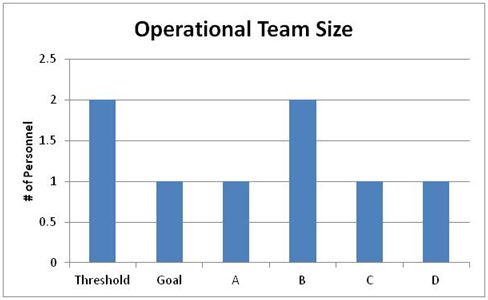
\includegraphics[scale=0.8]{images/operationalTeamSize.png}
	\end{center}
	\caption{Operational team size by variant}
	\label{fig:operationalTeamSize}
\end{figure}
\pagebreak

\section{Risk Analysis Data}
\label{sec:riskAnalysisData}
\begin{figure}[h!tbp]
	\begin{center}
		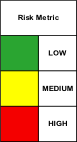
\includegraphics[scale=1]{images/riskMetricKey.png}
	\end{center}
	\caption{Risk metric key}
	\label{fig:riskMetricKey}
\end{figure}

\begin{figure}[h!tbp]
	\begin{center}
		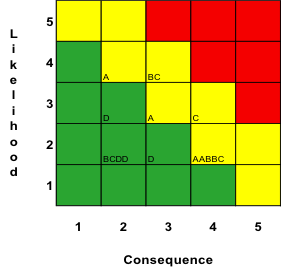
\includegraphics[scale=1]{images/riskAnalysisAll.png}
	\end{center}
	\caption{Risk analysis -- all variants}
	\label{fig:riskAnalysisAll}
\end{figure}

\begin{figure}[h!tbp]
	\begin{center}
		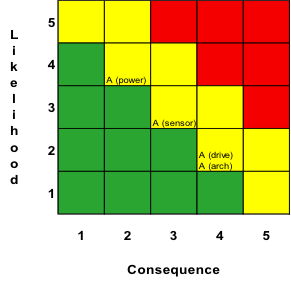
\includegraphics[scale=1]{images/riskAnalysisA.png}
	\end{center}
	\caption{Risk analysis -- variant A}
	\label{fig:riskAnalysisA}
\end{figure}

\begin{figure}[h!tbp]
	\begin{center}
		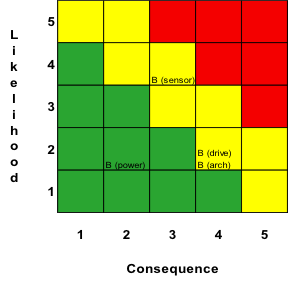
\includegraphics[scale=1]{images/riskAnalysisB.png}
	\end{center}
	\caption{Risk analysis -- variant B}
	\label{fig:riskAnalysisB}
\end{figure}

\begin{figure}[h!tbp]
	\begin{center}
		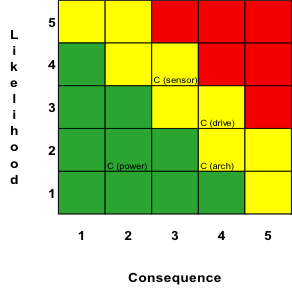
\includegraphics[scale=1]{images/riskAnalysisC.png}
	\end{center}
	\caption{Risk analysis -- variant C}
	\label{fig:riskAnalysisC}
\end{figure}

\begin{figure}[h!tbp]
	\begin{center}
		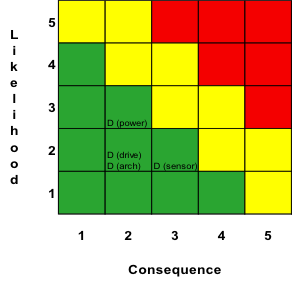
\includegraphics[scale=1]{images/riskAnalysisD.png}
	\end{center}
	\caption{Risk analysis -- variant D}
	\label{fig:riskAnalysisD}
\end{figure}

\end{document}
